%% Copyright 2019 Bernd Haberstumpf
%% License: CC BY-NC
% !TeX spellcheck = de_DE
\newchapter{Einleitung}\anchor{sec:rpg}

Der ``Operation P9''-Kampagne stellt ein eigenes, einfaches Rollenspiel-Regelwerk bereit. Die Werte der im vorherigen Kapitel vorgestellten Akteure basieren auf diesem Spielsystem. Nat"urlich kann auch ein der Rollenspielgruppe gel"aufigeres System verwendet werden.

\emph{Die folgenden Kapitel k"onnen den Spielern zur Verf"ugung gestellt werden. Die Kapitel stehen auch als ein separates, online verf"ugbares PDF-Dokument, die ``Spieler Referenz'', auf\newline{}\textit{https://github.com/poldi2015/Plane9} f"ur den Download bereit.}

\newchapter{Das C23-Universum}

Im Folgenden eine "Ubersicht "uber die relevanten Teile des C23-Universums als Vorbereitung und Nachschlagewerk f"ur die Spieler und den Spielleiter. Anschlie\3end wird das Regelwerk vorgestellt.

%% Copyright 2019 Bernd Haberstumpf
%% License: CC BY-NC
% !TeX spellcheck = de_DE
\newsection{Humanoide Rassen}

Neben nat"urlich oder k"unstlich befruchteten Menschen hat es die Menschheit vor einem halben Jahrhundert geschafft, Menschen die sogenannten Mutanten aus artifiziell sequenziertem Erbmaterial zu klonen. Das Erbmaterial der Mutanten ist auf das Leben au\3erhalb der Erde hin optimiert. Mutanten werden in Zuchtbottichen der gro\3en Konzerne gez"uchtet. Sie werden in Ausbildungskadern ohne eigene Eltern gro\3gezogen und f"ur ihre jeweilige Aufgabe ausgebildet. Mutanten haben ein gr"auliche Haut und keine K"orperbeharung. Mutanten stehen im Dienst diverser Gro\3konzerne sowie des terranen Milit"ars in einem leibeigenen Verh"altnis, aus dem sie sich unter Umst"anden freikaufen k"onnen. W"ahrend Mutanten auf der Erde angefeindet werden, sind sie in den au\3erterrestrischen Kolonien ein nat"urlicher Teil der Gesellschaft.

\begin{figure*}[htbp]
      \centering
      \fbox{
\includegraphics[width=0.75\textwidth]{images/cmyk/races_cmyk.jpg}}
      \newline{}Humanoide Rassen
      \label{fig:humanoide-rassen}
\end{figure*}
    

Im folgenden die relevanten Menschen und Mutantentypen.

\begin{description}
\item [Norms] Normal gebohrene Menschen werden Norms genannt. Seit der Besiedelung des Weltalls spielen die
      menschlichen Rassen keine so gro\3e Rolle mehr.
\item [Pure] Pure sind k"unstlich befruchtete, genetisch verbesserte Menschen. Das genetische Material wird vor der
      Befruchtung von negativen Genomen gereinigt. Pures sind Kinder der Superreichen und bilden einen signifikanten Teil der Oberschicht.
\item [Spacer] Spacer sind Humanoide, die ihr ganzes Leben in der Schwerelosigkeit verbracht haben. Bei Spacern haben
      sich Knochenmaterial und Muskel soweit zur"uck gebildet, dass sie sich nicht mehr ohne Exoskelett unter Schwerkraft wie auf der Erde oder dem Mars bewegen k"onnen. Stattdessen sind Spacer extrem geschickt in der Fortbewegung ohne Schwerkraft.
\item [Slags] Slags werden durch Strahlung mi\3gebildete Menschen genannt. Sie bilden den Bodensatz der
      humanen Gesellschaft.
\item [Alpha-Mutant] Alpha-Mutanten sind die als Arbeiter in den extraterrestrischen Kolonien konzipierten Mutanten.
      Alphas sind deutlich kr"aftiger als Norms und haben einen deutlich stabileren und massigeren K"orperbau. Alpha-Mutanten haben eine gro\3e Resistenz gegen kosmische Strahlung und sind gut ger"ustet f"ur unterschiedliche Schwerkraftbedingungen. Alpha-Mutanten sind schwere Arbeit unter gef"ahrlichen Bedingungen gew"ohnt und haben meist einen gutm"utigen Charakter.
\item [Eta Mutant] Etas sind als Piloten und Personal f"ur Raumschiffe konzipiert. Sie sind nur 1,35 bis 1,50 Meter gro\3
      und drahtig. Optimiert f"ur Schwerkraftextreme und erh"ohte kosmische Strahlung sind sie f"ur den Einsatz auf Raumschiffen optimal angepasst.
\item [Omega Mutant] Omega Mutanten sind als Infanterist im Armeedienst gez"uchtet. Sie sind 1,90 bis 2,10 Meter gro\3.
      Omegas sind "ahlich wie Alpha-Mutanten extrem kr"aftig und haben eine nahezu unzerst"orbare Konstitution. Omegas sind von klein auf f"ur den Kampf ausgebildet, haben taktische Erfahrung und kennen den Umgang mit allen Waffensystemen.
\end{description}

\newsection{Technologie}

Ein Gro\3teil der Shadowrun-Regeln, Cyberware und die Matrix als Virtuelle Realit"at k"onnen "ubernommen werden.

Im folgenden ein kleiner Auszug aus den spezieller Technologie der 23.~Jahrhunderts. Ideen f"ur weitere Technologie k"onnen aus anderen near Future Rollenspielen wie Shadowrun, Cyberpunkt, Alien etc.~"ubernommen werden.

\begin{description}
\item [ComLink] Ein ComLink wird zur drahtlosen Verbindung in das ComNetz genutzt. Das ComLink ist entweder als
      Mobilger"at mit AR Brille oder als Headware verf"ugbar.
\item [ComNetz] Ein ComNetz ist auf den meisten menschlichen Siedlungen etabliert. Das ComNetz ist eine virtuelle
      Computerwelt und Kommunikationsinfrastruktur. In das ComNetz bindet man sich per ComLink ein. Per Augmented Reality (AR) werden Informationen und Steuerelemente in das audiovisuelle Zentrum der Teilnehmer eingeblendet. Das ComNetz wird f"ur die Kommunikation, zur Informationsbeschaffung, f"ur Finanztransfers, zur Steuerung von Ger"aten etc.~genutzt. Um tiefer in das Netz einzutauchen und in einer vollsensorischen Virtuellen Realit"at einzutauchen, wird eine kabelgebundene Verbindung "uber eine Datenbuchse ben"otigt.
\item [Kontrollmodul] Das Kontrollmodul ist die Ankopplungszentrale an das Gehirn. Das Kontrollmodul erlaubt es Augmented Reality (AR)    
      Signale in das Sehzentrum und das H"ohrzentrum einzuspielen wie auch alle anderen Headware anzubinden.
\item [Credcard] Eine Credcard ist das Pendant zum ehemaligen Papiergeld. Eine vorher mit Geld aufgeladene Karte kann an
      einen Zahlungsempf"anger gegeben werden oder es kann per ComLink Geld von einer Credcard transferiert werden.
\item [Datenbuchse] Eine Datenbuchse ist eine am Hinterkopf verbaute Kabelschnittstelle zu einer Headware.
\item [Fusionstriebwerk] Fusionstriebwerke bilden den Hauptantrieb von Raumschiffen. "Uber Man"ovrierd"usen werden
      Raumschiffe in die richtige Positionen gebracht, um die m"achtigen Fusionstriebwerke zur Beschleunigung oder zum Abbremsen zu benutzen. Fusionstriebwerke nutzen eine Kernfusion mit HE-3 als Brennstoff und Wasser als Treibmasse.
\item [Headware] Mit dem Gehirn verbundene Hardware im Kopf, z.B.~ein ComLink das das ComNetz direkt mit dem Gehirn
      verbindet.
\item [ID-Chip] Menschen und Mutanten werden durch einen im linken Arm unter der Haut implantierten ID-Chip
      identifiziert. Der ID-Chip dient als Pass oder auch der Autorisierung von Zahlungen. Mittels Near-Field-Communication kann ein Reader auf den ID-Chip zugreifen.
\item [Magnetstiefel] Mangnetische Stiefel dienen dazu, in Schwerelosigkeit auf einem Raumschiff oder einer Station zu
      laufen. Zur Aktivierung werden sie zusammengeschlagen.
\item[PAN] Ein PAN (Personal Area Network) ist ein technisches System im Kopf der Person und umf"asst z.B.~ ein Kontrollmodul und   
      die Anbindungen des Girns an weitere Cyberware im K"orper wie auch angebundene Systeme au\3erhalb des K"orpers.
\item[Omni-Slate] Eine tragbare Workstation mit neuronaler Koppflung und Anbindungspunkte f"ur Steuerungseinheiten.
\item [Psychonauten] Psynchonauten sind Personen, die "uber eine kabelgebundene Verbindung das Gehirn
      einer anderen Person infiltrieren k"onnen. Dieser Gehirnscan erlaubt es, Gedanken, Erinnerungen und Gef"uhle des anderen zu erforschen. Da es sich um eine bidirektionale Verbindung handelt, erf"ahrt auch der Gescante evtl.~etwas "uber den Psychonauten. Ein Gehirnscan ist gef"ahrlich und kann zum Gehirntot der gescanten Person f"uhren.
\item [Raumanzug] Im 23.~Jahrhundert haben sich Raumanz"uge zu Tauchanz"ugen "ahnlichen Bodysuites entwickelt, die unter
      normaler Kleidung getragen werden k"onnen. Raumanz"uge sch"utzen vor Druck und Temperaturunterschieden. Zusammen mit Druckluftkanistern und Gesichtsmasken erlauben sie den Aufenthalt in Weltall.
\item [Riggersteuerung] Eine Riggersteuerug erlaubt es technische Ger"ate fern zu steuern. Die Riggersteuerung wird direkt im 
      Gehirn verbaut und mit dem Kontrollmodul verbunden oder extern "uber die Datenbuchse angebunden.
\item[Talentchip] Talentchips erweitern den Tr"ager "uber das Kontrollmodul um neue geistige und physische F"ahigkeiten. 
\end{description}

\newsection{Waffen}

Im folgenden ein Auszug von im 23.~Jahrhundert gebr"auchlichen Waffen.

\begin{description}
\item [Vibrokling] Eine durch hochfrequente Vibration extrem scharfe Klinge.
\item [Bolzenpistole] Ein Bolzenpistole ist eine semi automatische elektrisch getriebene Faustfeuerwaffe. Ein Bolzenpistole arbeitet "ublicherweise auf  
      dem Prinzip einer Railgun. Eine Railgun beschleunigt Hochgeschwindigkeitsprojektile entlang von zwei unter Strom gesetzten Stangen.
\item [Multigun] Eine Multigun in den meisten F"allen eine gro\3e Bolzenpistole, die es erlaubt zwischen     
      penetrierenden Projektilen und Schockmunition umzuschalten.
\item [Railgun Gewehr] Ein Railgun Gewehr oder kurz eine Railgun ist eine vollautomatische langl"aufige Version einer nach 
      dem Railgun Prinzip funktionierenden Faustfeuerwaffe. Railguns werden auch auf Schiffen als Verteidigung gegen anfliegende Geschosse genutzt.         
\item [Plasmaschleuder] Eine Plasmaschleuder ist eine Infanteriewaffe, die von Omega-Mutanten in einem Kampfpanzer zusammen mit
      einem R"uckentornister getragen wird. Die Plasmaschleuder verschie\3t hochenergetisches Plasma, das nahezu alles au\3er schweren Stahlplatten verbrennen kann.
\item [Raketenwerfer] Raketenwerfer sind eine der Hauptwaffensysteme von Raumschiffen.      
\item [Gefechtspanzer] Ein Gefechtspanzer ist ein Exoskelett mit starker Panzerung, eingebautem Raumanzug, Sensorik,
      Waffenplattformen und einem Jetpack. Ein Gefechtspanzer wird von Omega-Infanteristen eingesetzt.
\item [Gau\3kanone] Eine Gau\3kanone ist eine Waffensystem das auf Raumschiffen zum Einsatz kommt. "Uber mehrere Spulen
      werden Projektile in einem elektrisches Feld beschleunigt. Eine Gau\3kanone verschie\3t mit hoher Feuerrate Hochgeschwindigkeitsprojektile und gilt als die durchschlagskr"aftigste Feuerwaffe im Sonnensystem.         
\end{description}

\begin{figure*}[htbp]
      \centering
      \fbox{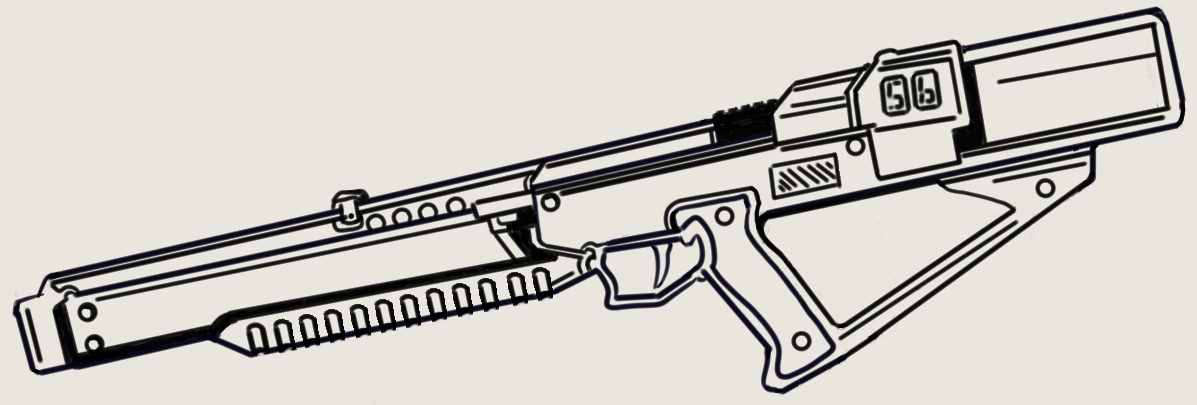
\includegraphics[width=0.75\textwidth]{images/railgun.png}}
      \newline{}Railgun
      \label{fig:rail-gun}
\end{figure*}

\newsection{Kommunikation}

Das jovianische System besitzt erst nach der Besiedelung durch das Protektorat eine nennenswerte Infrastruktur. Durch den rasanten Aufbau hat jedoch ein Gro\3teil der Einrichtungen einen provisorischen Charakter. Diese sind zudem auf das Notwendigste beschr"ankt. Das gilt auch f"ur die Kommunikations- und Informationssysteme. Wo auf Erde und Mars ein gutes ComNetz jegliche Information an jedem Punkt im System bereit stellt, steht ein voll ausgebautes ComNetz hier nur in Konzernsektoren und beim Milit"ar bereit.

Im jovianischen System  betreiben die einzelnen Monde und Stationen meist ein autonomes Kommunikationssystem, das mit den anderen Siedelungen und Anlagen nur in Teilen integriert ist. Ein ComNetz ist nur zwischen Monden und Stationen der Cynarian Corporation eingerichtet. Alle weitere Kommunikation zwischen Monden und Stationen erfolgt "uber Einzelverbindungen mittels der Sateliten rund um den Jupiter. Diese Verbindungen erlauben nur Kommunikation und Nachrichten zwischen Personen. Da die Stationen und Monde oft mehrere Millionen Kilometer voneinander entfernt sind, muss mit einer Kommunikationsverz"ogerung von mehreren Sekunden gerechnet werden.

Durch den steten unkontrollierten Zustrom von Mutantenfl"uchtlingen, Gl"ucksrittern und neuen Firmen stehen kaum Informationen zu Einzelpersonen und ans"assigen Institutionen und Unternehmen bereit.

\newsection{Fortbewegung und Reisezeiten}

Gro\3e Unternehmen wie Cynarian, das Protektoratsmilit"ar und die Protektoratsadministration betreiben eigene Shuttleflotten innerhalb des Systems soweit n"otig. Einige wenige Personen besitzen ebenfalls Shuttles. Der Rest der Fl"uge zwischen den Jupitertrabanten wird durch Transportunternehmen und Schiffseignern von Shuttles bereitgestellt. Einen Flug bekommt man am einfachsten im Raumhafen der jeweiligen Station. Die Reisen im Jovianischen System dauern ja nach Konstellation der Monde 1-2 Tage.

%% Copyright 2019 Bernd Haberstumpf
%% License: CC BY-NC
% !TeX spellcheck = de_DE
\newchapter{Einf"uhrung}

\newsection{Vorgeschichte}

Durch ein menschenverachtendes Vorgehen von k"unstlichen Intelligenzen beim Kampf gegen die Mutantenrebellion sind KIs zum wiederholten Mal in den Augen der Menschheit in Ungnade gefallen. Da die Cynarian Corporation f"ur den Aufbau einer Industrie auf dem Jupiter enorme Ressourcen ben"otigt, nimmt das Unternehmen die aktuelle Stimmung zum Anlass, um unter anderem die vielversprechende aber teure KI-Forschungsabteilung unter der Leitung von \emph{Prof.~Dr.~Naratova} auf der Mars \emph{Orbitalstation Neu-Gr{\o}ning} zu streichen.

Im Zuge der Besiedelung des Jupiter wird Neu-Gr{\o}ning daraufhin zum Jupiter geschleppt und als \emph{Nike Station} zum Verwaltungs- und F\&E St"utzpunkt der Cynarian Corporation im Jovianischen System eingerichtet. Neben Forschungslaboren unter der Schirmherrschaft der Cynarian Corporation werden auch Einrichtungen von Zulieferfirmen auf Nike zugelassen. F"uhrende Mitarbeiter der ehem.~KI-Abteilung gr"unden daraufhin unter der Leitung von Prof.~Dr.~Naratovas den unabh"angigen Headware Zulieferer \emph{Neuro Intelligence} unter anderem auch mit Geldern aus Tarnfirmen der United Space Industries. Die Labore und Produktionsst"atten der Neuro Intelligence werden in alten R"aumlichkeiten der ehemaligen KI-Abteilung auf Ebene 9 der Nike Station eingerichtet. Neuro Intelligence beliefert im Jovianischen System die Kliniken auf dem Mond Kallisto mit neuronaler Soft- und Hardware. Da die Implantate, die die Neuro Intelligence im Auftrag der Kliniken fertigt, Ma\3anfertigungen sind, erh"alt Neuro Intelligence weitreichende Informationen "uber die zuk"unftigen Tr"ager der Implantate.

Seit der Gr"undung entwickelt Neuro Intelligence im geheimen Auftrag mit Geldern und Technologie des USI-Geheimdienstes KI-Implantate unter dem Decknamen \hl{Operation P9}. Dabei gelingt es, die KI symbiotisch mit dem menschliche Gehirn zu verbinden und damit der KI je nach Auspr"agung die "Ubernahme des Tr"agers zu erlauben. Nicht jedes Gehirn ist f"ur die "Ubernahme geeignet. Inwieweit das Gehirn und die KI eine Symbiose eingehen, ist nicht bekannt. In der ersten Erprobung werden nur die Gehirne von Mutanten manipuliert. Die Einbringung der KI erfolgt durch ein modifiziertes \emph{Kontrollmodul}, der neuronalen Schnittstelle ins Gehirn, in das die KI eingebettet ist. Die KI selbst ist ein Verbund aus autonomen Nanobots, die sich im Gehirn automatisch verbreiten und sich mit den Synapsen des Gehirns verbinden.

\newsection{Chronologie der Attentate}\anchor{sec:assassinations}

Mit Hilfe von durch KIs manipulierte Mutanten startet die USI als Feldtest eine Anschlagsreihe auf das Protektorat um die Stellung des Potektorats und die der Cynarian Corporation zu diskreditieren.

Bevor die Charaktere in das Spielgeschehen eingebunden werden, hat es bereits mehrere Vorf"alle im Jovianischen System gegeben, die teils auf Attentate zur"uckzuf"uhren sind:

\begin{description}
\item [Vor 10 Wochen] Shuttleabsturz durch Pilotenfehlverhalten auf dem Hangardeck der Minenkolonie \emph{Hellgate}. Vom Shuttle Absturz 
      erfahren die Ermittler erst durch Nachforschungen auf Hellgate. Bei dem Shuttleabsturz handelt es sich um kein Attentat.
\item [Vor 9 Wochen] Fehlfunktion eines Minenschleppers der Hellgate Station durch fehlerhaft programmierte Steuerungskomponenten. Die 
      Reparatur dauert noch an. Der verantwortliche Ingenieur kann nicht festgestellt werden. "Uber die Schlepperfehlfunktion wird der Cynarian Ermittler beim ersten Briefing aufgekl"art. Das Attentat wurde durch den Alpha-Mutanten \emph{Hannibal} durchgef"uhrt der allerdings bereits zwei Wochen vor dem Schlepperunfall auf die Mine HeM03 versetzt wird.      
\item [Vor 7 Wochen] Die \emph{Mine HeM03} auf dem Jupiter wird zerst"ort. Ein Teil der Besatzung kann mit dem  Rettungsschuttle fliehen. 
      Als mutma"sliche Attent"aterin gilt die Alpha-Mutantin \emph{Sent} die bei dem Attentat get"otet wird. Beim eigentlichen Attent"ater handelt es sich ebenfalls um den Alpha-Mutant Hannibal der mehrere Minenarbeiter sowie Sent t"otet. "Uber den Minenunfall werden beide Chefermittler w"ahrend ihres ersten Briefings informiert.
\item [Vor zwei Wochen] Explosion beim Anbau von neuen Habitaten an den "au\3eren Ring des Armageddon Raumkomplexes. Zug"ange und ein
      ehemaliger Frachter, der als Habitat dienen sollte, werden stark besch"adigt.  Es gibt mehrere Tote. Ursache ist eine Fehlfunktion einer Drohne. Der Attent"ater \emph{Slingshot} wird als solcher nicht erkannt. "Uber den Unfall auf Armageddon wird der Chefermittler des Protektorats bei der Besprechung mit Avenger aufgekl"art.
\item [Vor drei Tagen] Havarie der Mine HeM05. Die mutma\3liche Attent"aterin, eine Mutantin mit dem Namen \emph{Pitch}, hat das
      Rettungsshuttle sabotiert und 3 von 5 Tr"agerballons zerst"ort. Danach st"urzt sie von der Galerie der Mine in den Abgrund. Die Mine kann durch den heldenhaften Einsatz von J"agern der Hellgate Station und mit Hilfe eines Minenschleppers gerettet und zur Hellgate Station gebracht werden. W"ahrend der Einsatzbesprechung der Ermittler sitzen die geretteten Minenarbeiter noch in einer Dekompressionskammer. "Uber die Sabotage werden beide Chefermittler w"ahrend ihres ersten Briefings informiert. Der eigentliche
      T"ater ist wie bei Mine HeM03 der Alpha-Mutant Hannibal, der zusammen mit den anderen "Uberlebenden gerettet wird.
\end{description}

\newsection{Die Charaktere}

Die Charaktere "ubernehmen die Rolle der Ermittler, die die Attentatsreihe aufkl"aren sollen. Die Kampagne sieht zwei Ermittler aus den Reihen der Cynarian Corporation und zwei Ermittler aus den Reihen des Protektorats vor. Beide Gruppen sind jeweils ihren eigenen Organisationen verpflichtet und sollten entsprechend handeln (ggf.~durch entsprechende W"urfelw"urfe einfordern).

Cynarian stellt einen Chefermittler und einen Assistenten bereit. Der Protektor stellt einen Chefermittler und einen Angeh"origen des Protektoratsmilit"ars bereit. Wird die Kampagne nur mit drei Spielern gespielt, entf"allt die Rolle des Cynarian Unterst"utzers und der Chefermittler "ubernimmt seine Rolle. Die F"uhrung der gesamten Operation "ubernimmt dann der Chefermittler des Protektorats. 

\newsubsection{Cynarian, Chefermittler}
Beim Chefermittler der Cynarian Corporation sollte es sich um einen Norm, einen Mensch mit F"uhrungsqualit"aten und Ermittlererfahrung handeln. Denkbar ist zum Beispiel der Kommandant eines Raumschiffs aus dem Asteroideng"urtel zwischen Mars und Jupiter auf der Jagd nach Piraten. Der Chefermittler der Cynarian Corporation sollte als Milit"arangeh"origer klar den Anweisungen der Corporation folgen, auch wenn das bedeutet der Gruppe Informationen vorzuenthalten oder sonstig im Sinne des Konzerns zu handeln.

\newsubsection{Cynarian, assistierender Ermittler}
Der Assistent ist ein \emph{Psychonaut}, ein Mensch mit spezieller Ausbildung, der in die Gedanken einer anderen Person "uber eine Kopf zu Kopf Datenverbindung eintauchen kann. Er sollte als Konzern- oder auch als freier Agent auftreten. Der Assistent sollte versuchen seine spezielle F"ahigkeit vor der Gruppe geheim zu halten und nur die Konzernspitze "uber die detaillierten Ergebnisse seiner Untersuchungen informieren. Der Assistent sollte ein Norm sein.

\newsubsection{Protektorat, Chefermittler}
Der Chefermittler des Protektorats sollte ein Vertrauter des Protektors Avenger und dessen Stabs sein. Er k"onnte sich z.B.~um den Betrieb Armageddons und die Aufnahme von neuen Bewohnern, Fl"uchtlingen von der Erde, k"ummern. Er hat Ortskenntnisse und weitreichende Kontakte im Mutantenteil des jovianischen Systems. Der Chefermittler mu\3 deshalb ein Alpha-Mutant sein. Der Chefermittler des Protektorats hat das Wohlsein der Mutanten als pers"onliche Mission im Blut. Auch sollte er dem Herrscheranspruch des Protektoratsmilit"ars kritisch gegen"uber stehen.

\newsubsection{Protektorat, assistierender Ermittler}
Der Assistent wird durch das Protektoratsmilit"ar gestellt und hat somit einen milit"arischen Hintergrund. Er ist ein \emph{Omega}, ein Kampfmutant. Sollte er sich von den Cynarian Mitarbeitern befehligt oder hintergangen f"uhlen w"urde er darauf reagieren. Direkte Anweisungen von Konzernmitarbeitern wird er nicht akzeptieren, wenn es eine Konfliktsituation nicht unbedingt erforderlich macht. Die Omega-Krieger f"uhlen sich dem Rest der Welt in Sachen St"arke und Willenskraft "uberlegen. Er misstraut Norms und den Konzernen und h"alt die zivilen Einrichtungen des Protektorats f"ur zu nachgiebig.

Inwieweit die Gruppe die vorprogrammierten Spannungen zwischen den Charakteren ausspielt, bleibt der Gruppe vorbehalten. Die Aufgabe des Spielleiters ist es, die Balance zu halten, um den Plot nicht zu gef"ahrden und stattdessen vorantreiben zu k"onnen. 
%% Copyright 2019 Bernd Haberstumpf
%% License: CC BY-NC
% !TeX spellcheck = de_DE
\newsection{Regelsystem}\anchor{sec:rules}

Die Rollenspielregeln sind auf den narrativen Charakter des Plots ausgelegt. Es handelt sich um ein W6 W"urfelsystem bei dem vier W"urfel pro Spieler bzw.~den Spielleiter ausreichen. W"urfel legen dabei nicht die Eigenschaften einen Charakter im Detail fest oder beschreiben das Ergebnis einer Aktion, sondern speisen lediglich einen Zufallsfaktor in das Ergebnis ein. Das Ergebnis einer Aktion oder auch eines Ereignisses legt der Spielleiter unter Ber"ucksichtigung der Handlungen und des W"urfelergebnisses selbst fest. Das Regelsystem ist in Teilen inspiriert durch das Rollenspiel ``Blades in the Dark''.

%% Copyright 2019 Bernd Haberstumpf
%% License: CC BY-NC
% !TeX spellcheck = de_DE
\newsection{W"urfelw"urfe}

Der Erfolg einer \emph{Aktion} wird, wie beschrieben, durch W"urfel beeinflusst. Das W"urfelergebnis bestimmt, wie erfolgreich eine Aktion gewesen ist. W"urfelw"urfe werden mit einem bis f"unf W6-W"urfeln durchgef"uhrt, wobei das h"ochste W"urfelergebnis, beziehungsweise die h"ochsten W"urfelergebnisse z"ahlen.

Es wird zwischen den folgenden Schwierigkeitsgraden unterschieden: \emph{``Alltagswurf''}, \emph{``Einfacher Wurf''}, \emph{``Risikowurf''} und \emph{``Vergleichender Wurf''}.

\newsubsection{Alltagswurf}
Ein ``Alltagswurf'' kann bei einer allt"aglichen Situation zum Einsatz kommen. Eine allt"agliche Situation ist z.B. eine Suche im ComNetz. Bei einem Alltagswurf werden drei W"urfelergebnisse unterschieden:

\begin{diceroles}
    \sdice{1} & Die Aktion ist fehlgeschlagen, oder dem Ausf"uhrenden ist m"oglicherweise sogar ein Missgeschick unterlaufen.\\
    \rdice{2}{5} & Die Aktion hat Erfolg. \\
    \sdice{6} & Die Aktion hat einen herausragenden Erfolg. \\
\end{diceroles}

\begin{ruleexample}
    Rondra ist auf der Suche nach Informationen in einer einschl"agigen Diskothek. Sie begibt sich erst einmal auf die Tanzfl"ache. Der Spielleiter entscheidet sich f"ur einen Alltagswurf. Rondra w"urfelt:

    \begin{diceroles}
        \sdice{1} & Rondra rempelt mehrere Discobesucher an und ger"at damit ins Visier der T"ursteher.\\
        \rdice{2}{5} & Rondra tanzt ungezwungen und kann dabei andere Discobesucher ansprechen. \\
        \sdice{6} & Rondra legt eine beeindruckende Performance aufs Parkett und erregt das Interesse des Barmanns Bruno, der ihr nur 
            allzu gerne Antworten auf ihre Fragen gibt.\\
    \end{diceroles}
\end{ruleexample}

\newsubsection{Einfacher Wurf}
Ein ``Einfacher Wurf'' beeinflusst das Ergebnis einer nicht allt"aglichen Herausforderung. Folgende W"urfelergebnisse werden unterschieden:

\begin{diceroles}
    \sdice{1} &  Die Aktion ist fehlgeschlagen und hat negative Auswirkungen.\\
    \rdice{2}{3} & Die Aktion hat keinen Erfolg. \\
    \rdice{4}{5} & Die Aktion hat einen Teilerfolg. \\
    \sdice{6} & Die Aktion hat vollen Erfolg.\\
    \tdice{6}{6} & Die Aktion hat einen herausragenden Erfolg.\\
\end{diceroles}

\begin{ruleexample}
    Hektor ist auf der Suche nach Informationen im Raumhafen von Valhalla. Er wird von dem Agenten Johnson beschattet. Der Spielleiter l"asst den Spieler w"urfeln. Wird er den Agenten als solchen erkennen?

    \begin{diceroles}
        \sdice{1} & Der Agent rempelt Hektor unerkannt an und heftet ihm eine Nanowanze an den Overall.\\
        \rdice{2}{3} & Hektor bemerkt nichts.\\
        \rdice{4}{5} & Hektor bemerkt, dass er verfolgt wird verliert den Agenten aber zun"achst wieder aus den Augen.\\
        \sdice{6} & Hektor hat den Agenten entdeckt, ohne das dieser seine Entdeckung bemerkt hat.\\
        \tdice{6}{6} & Hektor hat den Agenten entdeckt und schafft es ihn auf eine falsche F"ahrte zu locken.\\
    \end{diceroles}
\end{ruleexample}

\newsubsection{Risikowurf}
Ein ``Risikowurf'' ist ein W"urfelwurf, bei dem der W"urfelnde geringe Chancen auf Erfolg hat. Folgende W"urfelergebnisse kommen in Betracht:

\begin{diceroles}
    \sdice{1} & Die Aktion ist fehlgeschlagen und hat negative Auswirkungen.\\
    \rdice{2}{5} & Die Aktion hat keinen Erfolg.\\
    \sdice{6} & Die Aktion hat einen Teilerfolg erzielt.\\
    \tdice{6}{6} & Die Aktion hat einen vollen Erfolg.\\
    \hdice{6}{6}{6} & Die Aktion hat einen herausragenden Erfolg.\\
\end{diceroles}

\begin{ruleexample}
    In einem Raumgefecht erleidet Hektors Shuttle einen Schaden an der Steuereinheit und taumelt durchs All. Hektor beschlie\3t, den Schaden an der Bordwand zu reparieren, und verl"asst im Raumanzug das Innere des Schiffs. Der Spielleiter l"asst w"urfeln:
    
    \begin{diceroles}
        \sdice{1} & Hektors Magnetstiefel verlieren die Haftung auf der Bordwand und er schl"agt mit dem Kopf auf. Nun h"angt er          
            bewusstlos am Rettungsseil. Hoffentlich ist noch eine zweite Person an Bord, die ihn retten kann.  \\
        \rdice{2}{5} & Hektor kann den Schaden nicht beheben.\\
        \sdice{6} & Hektor schafft es, einen Teil der Steuereinheit notd"urftig zu reparieren. Hoffentlich reicht es, das Schiff aus        
            der Schusslinie zu bringen.\\
        \tdice{6}{6} & Hektor kann die Steuereinheit wieder in Betrieb nehmen.\\
        \hdice{6}{6}{6} & Hektor repariert die Steuereinheit und koppelt sie gleich noch mit der Waffenkontrolle.\\
    \end{diceroles}
\end{ruleexample}

\newsubsection{Vergleichender Wurf}
Ein ``Vergleichender Wurf'' ist ein regul"arer Wurf, bei dem die Anzahl der verf"ugbaren W"urfel und der Schwierigkeitsgrad durch Aktionen eines ``Gegners'' negativ beeinflusst werden k"onnen.

Die Anzahl der W"urfel, die f"ur eine Aktion bereitstehen, wird durch die Anzahl der W"urfel, die dem Gegner f"ur seine Aktion zur Verf"ugung stehen, reduziert.

\begin{itemize}
    \item Aktionsw"urfel +1 werden um die Anzahl der W"urfel des Gegners reduziert.
    \item Resultat $\leq$ 0 erh"oht die Schwierigkeit.
    \item Es wird mit mindestens einem W"urfel gew"urfelt.
\end{itemize}

Wenn weniger als ein W"urfel "ubrig bleibt, wird mit einem W"urfel gew"urfelt und es erh"oht sich die Schwierigkeit nach folgender Tabelle:

\begin{center}\begin{tabular}{m{3cm} m{5.5ex} m{3.5cm}}
    \textbf{Schwierigkeit} & \textbf{wird} & \textbf{Schwierigkeit} \\\hline
    Alltagswurf            & $\rightarrow$ & Einfacher Wurf \\
    Einfacher Wurf         & $\rightarrow$ & Risikowurf \\
    Risikowurf             & $\rightarrow$ & Risikowurf \\
\end{tabular}\end{center}

\underline{Anmerkung:} Vergleichende W"urfe kommen vor allem bei K"ampfen zum Einsatz. Im Kampf bedeutet dies, dass ein Charakter ohne Kampferfahrung gegen einen kampferfahrenen Gegner immer einen Risikowurf w"urfelt.

\medskip
\begin{ruleexample}
    Hektor verfolgt den Agenten Johnson in den Raumhafen. Johnson ist sich der Gefahr bewusst und will sich der Verfolgung entziehen. Der Spielleiter entscheidet sich f"ur einen Vergleichenden Wurf mit der Schwierigkeit Einfacher Wurf.

    \underline{Reduzierte W"urfel}

    Hektor stehen regul"ar zwei W"urfel zur Verf"ugung. Dem Agenten stehen f"ur sein Versteck auch zwei W"urfel zur Verf"ugung. Hektors W"urfelanzahl wird um einen W"urfel reduziert (Hektors W"urfel +1 minus W"urfel des Gegners). Die Schwierigkeit erh"oht sich nicht, da nach Abzug der gegnerischen W"urfel immer noch ein W"urfel zur Verf"ugung steht.

    \underline{Erh"ohte Schwierigkeit}

    Hektor stehen regul"ar zwei W"urfel zur Verf"ugung. Der Agent ist ein Meister der Tarnung und hat drei W"urfel zur Verf"ugung. Hektors W"urfelanzahl w"urde auf null reduziert. Die Schwierigkeit, den Agenten zu entdecken, steigt auf Risikowurf. Hektor w"urfelt mit einem W"urfel.
\end{ruleexample}

\newsubsection{Kr"afte B"undeln}\anchor{sec:bundleforce}
Bei einer Aktion k"onnen mehrere Personen ihre Kr"afte b"undeln, um ihre Erfolgschancen zu erh"ohen. Das B"undeln ist jedoch nur dann m"oglich, wenn die Spieler glaubhaft erkl"aren k"onnen, wie sie gemeinsam eine Aktion ausf"uhren.

Beim B"undeln einer Aktion werden die W"urfel aller beteiligten Personen einschlie\3lich Boni zusammen addiert. Die maximale Anzahl der W"urfel ist auf f"unf W"urfel, ohne Boni auf drei W"urfel begrenzt. Bei einem vergleichenden Wurf wird die maximale Anzahl an W"urfeln \emph{nach} Abzug der gegnerischen W"urfel auf die maximal zul"assige Anzahl beschr"ankt. B"undeln die Gegner ebenfalls ihre W"urfel, wird die geb"undelte Anzahl an W"urfeln des Gegners abgezogen.

\medskip
\begin{ruleexample}
    Hektor und Rondra versuchen, einen guten Preis f"ur den Flug auf dem Frachter "`Leviathan"' von Valhalla zum Mars auszuhandeln. Der Eigner Dudelwald und seine Frau Sandmann halten dagegen. Beide Gruppen nutzen die F"ahigkeit \stat{Communication} und b"undeln ihre Kr"afte. Hektor hat nur einen W"urfel zur Verf"ugung, Rondra dagegen zwei. Die beiden Eigner haben jeweils einen W"urfel zur Verf"ugung. Hektor und Rondra gehen also mit drei W"urfeln ins Rennen, von denen ein W"urfel abgezogen wird (die Eigner haben $1+1$ W"urfel minus ein W"urfel zur Berechnung den Vergleichenden Wurf). Damit k"onnen Hektor und Rondra zumindest einen Wurf mit zwei W"urfeln durchf"uhren.
\end{ruleexample}

%% Copyright 2019 Bernd Haberstumpf
%% License: CC BY-NC
% !TeX spellcheck = de_DE
\newsection{Der Charakter}\anchor{sec:character}

Die F"ahigkeiten und Eigenschaften eines Charakters sind, neben den menschlichen Grundf"ahigkeiten, durch seinen Hintergrund und spezielle St"arken und Schw"achen bestimmt. 

\begin{description}
    \item[Grundf"ahigkeiten] Grundf"ahigkeiten sind F"ahigkeiten die jeder Humanoiden mehr oder weniger beherrscht. Alles, wof"ur keine
        spezielle Ausbildung, kein spezielles ethnischer oder kulturelles Hintergrundwissen und keine speziellen K"orpereigenschaften ben"otigt werden, f"allt in diese Kategorie. Jeder der es bis ins All geschafft hat, kann lesen, schreiben und rechnen. Auch kann jeder eine entsicherte Feuerwaffe abfeuern. Alle Bewohner der au\3er terrestrischen Kolonien k"onnen sich miteinander irgendwie unterhalten. Gesprochen wird ein Kauderwelsch aus Englisch mit starken Einfl"ussen von Russisch, Chinesisch und Spanisch. Ausfl"uge mit einem Raumanzug ins All sind hingegen nicht selbstverst"andlich. Aktionen in einer Grundf"ahigkeit werden mit \textbf{1W6} gew"urfelt. 
    \item[Hintergr"unde] Hintergr"unde beginnen mit einer Kulturkreis entsprechender Muttersprache, fortgef"uhrt durch Schulbildung und 
        Profession mit entsprechendem Wissen und entsprechenden F"ahigkeiten wie auch Kontakten. Der Hintergrund erweitert Grundf"ahigkeiten des Charakters individuell. Hintergr"unde werden ebenfalls mit \textbf{1W6} gew"urfelt. Was die Hintergr"unde eines Charakters umfassen kann in Szenen individuell durch den Spielleiter passend zum Spielverlauf bestimmt werden. Kann der Spieler aufgrund seines Hintergrunds glaubhaft darlegen, dass er eine F"ahigkeit beherrscht, kann er diese auch anwenden.
    \item[St"arken] St"arken beschreiben was ein Charakter besonders gut kann. St"arken erlauben es mit zus"atzlich auf entsprechende 
        Aktionen zu w"urfeln. 
    \item[Talente \& Schw"achen] Talente sind besondere Eigenschaften wie eine fotografisches Ged"achtnis. Schw"achen k"onnen k"orperliche  
        Gebrechen, Phobien, eine Sucht aber auch eine rachs"uchtige Exfreundin sein. Sie k"onnen durch den Spielleiter oder auch vom Spieler eingesetzt werden, um dem Charakter mehr pers"onlichen Tiefgang zu geben.
\end{description}        

%% Copyright 2019 Bernd Haberstumpf
%% License: CC BY-NC
% !TeX spellcheck = de_DE
\newsection{Die Helden}\anchor{sec:helden}

Eine Rollenspielkampagne entspricht einer Actionserie, bei der die Spieler die Rollen der Helden "ubernehmen. Als Held treten die Charaktere aus der Masse der Normalsterblichen heraus. Helden k"onnen ausweglose Situationen meistern, denn sie haben \emph{Gl"uck}, mehr Gl"uck als normale Personen. 

\begin{column}[l]{0.52}
    Im Regelwerk wird das Gl"uck durch Schicksalspunkt, \stat{FATE} auf dem Charakterblatt repr"asentiert, die w"ahrend des Spiels ausgegeben werden k"onnen.
\end{column}
\begin{column}[r]{0.48}
    \centering
    
\includegraphics[width=0.80\textwidth]{images/character_fate.png}    
\end{column}

Schicksalspunkte werden nach jeder Szene wieder aufgef"ullt. Das Ausgeben eines Schicksalspunktes, erlaubt es dem Spieler, einen oder mehrere \textbf{W"urfel noch einmal zu w"urfeln oder} alternativ \textbf{einen W"urfel zus"atzlich} zu werfen. Ein W"urfelwurf darf dabei allerdings maximal mit vier W"urfeln, bei Anwendung von Waffen- oder R"ustungensbonus mit f"unf W"urfeln ausgef"uhrt werden. F"ur jede Aktion darf nur maximal ein Schicksalspunkt ausgegeben werden. F"ur jeden ausgegebenen Schicksalspunkt wird ein K"astchen unter FATE abgestrichen.

Die Helden sind im Normalfall keine ungebildeten Tagel"ohner. Sie besitzen eine gute Ausbildung, Kontakte und Ressourcen. K"orpermodifikationen wie ein Kontrollmodul d"urfen vorausgesetzt werden. Helden sind zumindest rudiment"ar mit dem Umgang eines Raumanzugs vertraut.

Helden sind z"ah. Wie in einem Roman stehen Helden in jeder neuen Szene auf der Matte, um die n"achste Herausforderung zu meistern. Die Szenen in einer Geschichte sind meist so gestaltet, dass dazwischen Zeit vergeht und die Charaktere sich in einer sicheren Umgebung aufhalten k"onnen. So k"onnen sie sich erholen. Verletzungen, die ein Weiterspielen behindern oder unglaubw"urdig machen, k"onnen in einer sicheren Umgebung geheilt werden. Die Medizin hat sich in den zuk"unftigen 200 Jahren stark weiterentwickelt. KI gest"utzte Autobots assistieren bei medizinischen Eingriffen oder f"uhren Operationen selbst durch. Innere Organe lassen sich durch k"unstliche Organe ersetzen. Gez"uchtete und k"unstliche Gliedma\3en lassen nat"urliche Gliedma\3en voll funktionsf"ahig ersetzen. Mikrobenkulturen erlauben, Verletzte zu stabilisieren.

%% Copyright 2019 Bernd Haberstumpf
%% License: CC BY-NC
% !TeX spellcheck = de_DE
\newsection{Charakter Erschaffung}

Die F"ahigkeiten und Eigenschaften eines Charakters werden bei der Erstellung des Charakters festgelegt und auf seinem Charakterdatenblatt festgehalten. Das Charakterdatenblatt ist am Ende dieses Kapitel angeh"angt. Es kann auch separat im Internet heruntergeladen werden. Ein entsprechender Link findet sich unter Quellenangaben am Ende des Buchs. Charakterdatenbl"atter sind "ublicherweise, wie auch bei diesem Regelsystem, in englischer Sprache verfasst.

\newsubsection{Allgemeine Daten}
\begin{column}[l]{0.48}
    Das Charakterdatenblatt beginnt mit allgemeinen Daten wie Name, Geschlecht (\stat{GENDER}), Rasse (\stat{RACE}), Alter (\stat{AGE}), Talente und Schw"achen (\stat{MERITS \& FLAWS}). Die verf"ugbaren Rassen sind im n"achsten Kapitel beschrieben.
\end{column}
\begin{column}[r]{0.52}
    \centering
    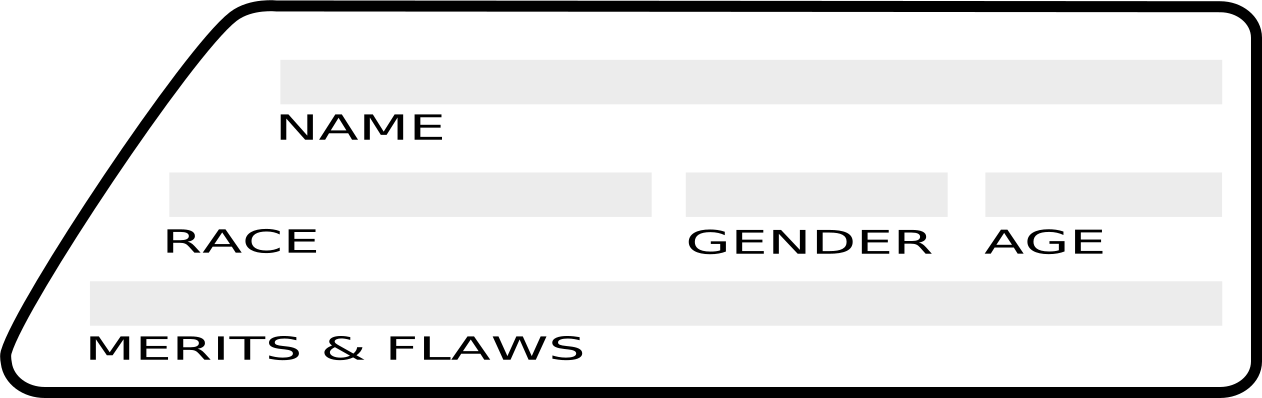
\includegraphics[width=0.95\textwidth]{images/character_base_stats.png}
    \medskip   
\end{column}
\medskip

\sheet{Name, Geschlecht, Rasse und Alter k"onnen durch den Spieler frei gew"ahlt werden.}

Die Charaktere sind "ublicherweise zwischen 30 und 50 Jahre alt. Ein deutlich niedriges oder deutlich h"oheres Alter kann negative Einfl"usse auf k"orperliche Verfassung oder die F"ahigkeiten des Charakters haben. Eine Einschr"ankung kann unter \stat{MERITS \& FLAWS} auf dem Charakterdatenblatt notiert werden.

\sheet{Um die Charaktere dar"uber hinaus lebhafter zu gestalten, kann eine Schw"ache, ein Flaw, f"ur den Charakter festgelegt werden.}

\newsubsection{Hintergrund}
\begin{column}[l]{0.52}
    Die \cref{sec:character} eingef"uhrten Hintergr"unde des Charakters werden im Feld \stat{BACKGROUND} notiert. Die Hintergr"unde beschreiben den individuellen Lebensweg eines Charakters.
\end{column}
\begin{column}[r]{0.48}
    \centering
    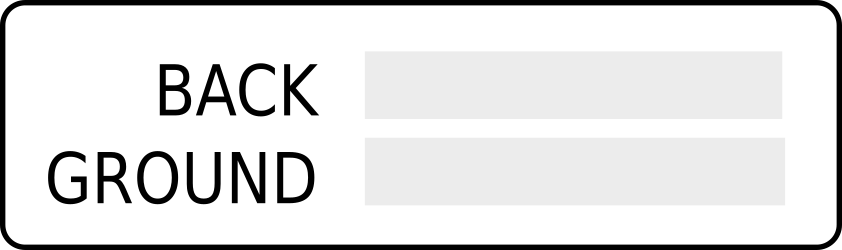
\includegraphics[width=0.80\textwidth]{images/character_background.png}    
\end{column}

\medskip
Hintergr"unde sind jeweils einem der \emph{Attribute} \stat{[B]ODY}, \stat{[E]MPATHY} und \stat{E[D]UCATION} zugeordnet. Die einem Attribut zugeordneten St"arken, die sogenannten \emph{F"ahigkeiten}, beziehen sich immer auf entsprechende Hintergr"unde.

\sheet{Das Attribut, auf das sich ein Hintergrund bezieht, wird in der Hintergrundbeschreibung unter \stat{BACKGROUND} mit \stat{[B]}, \stat{[E]} oder \stat{[D]} erg"anzt.}

\medskip
\begin{ruleexample}
    Bei einem Agenten der Cynarian Corporation findet sich z.B. der \stat{BACKGROUND} "`Cynarian Agent [E]"', wobei \stat{[E]} das Attribut \stat{[E]MPATHY} kennzeichnet. St"arken im Bereich des Attributs sind auf das Umfeld eines Cynarian Agenten beschr"ankt.
\end{ruleexample}

\newsubsection{Attribute und F"ahigkeiten}
Die St"arken eines Charakters werden aufgeteilt nach den Attributen \stat{[B]ODY}, \stat{[E]MPATHY} und \stat{E[D]UCATION} gruppiert. Die Attribute repr"asentieren die Grundf"ahigkeiten des Charakters. Unter den Attributen sind die St"arken, die sogenannten \emph{F"ahigkeiten} des Charakters gruppiert. Jedem Attribut sind jeweils drei F"ahigkeiten zugeordnet. 

Neben einer F"ahigkeit ist jeweils die Anzahl der W"urfel notiert, die f"ur eine Aktion zur Verf"ugung stehen. F"ur die F"ahigkeiten eines Charakters stehen bis zu drei W"urfel zur Verf"ugung, die durch die Boxen neben den F"ahigkeiten  festgehalten werden. Die erste bereits ausgef"ullte Box neben jedem Attribut und jeder F"ahigkeit symbolisiert, dass f"ur beliebige Aktionen mindestens ein W"urfel zur Verf"ugung steht.

Ein gef"ulltes Dreieck rechts neben einem Attribut zeigt an, dass f"ur die darunterliegenden F"ahigkeiten bis zu drei W"urfel zur Verf"ugung stehen k"onnen. Bei Attributen mit leerem Dreieck stehen maximal zwei W"urfel f"ur eine F"ahigkeit zur Verf"ugung. Bei Mutanten ist das Dreieck bei \stat{BODY} ausgef"ullt. Norms k"onnen frei zwischen \stat{EMPATHY} und \stat{EDUCATION} w"ahlen.

Bei der Charaktererstellung k"onnen f"ur F"ahigkeiten insgesamt 6 Punkte vergeben werden. F"ur jeden ausgegebenen Punkt kann eine Box neben einer F"ahigkeit ausgef"ullt und damit ein zus"atzlicher W"urfel erworben werden.

\newsubsection{F"ahigkeiten}
Die 9 F"ahigkeiten beschreiben grob die St"arken eines Charakters. Inwieweit eine F"ahigkeit auf eine Aktion anwendbar ist, liegt im Ermessen des Spielleiters. Die F"ahigkeiten sind bewusst allgemein gehalten und k"onnen sich "uberschneiden. Der Spieler beschreibt zun"achst die Aktion, die er ausf"uhren will. Anschlie\3end bestimmen der Spieler und der Spielleiter gemeinsam, welche F"ahigkeit am besten anwendbar ist.

Die F"ahigkeiten eines Charakters beziehen sich immer auf einen entsprechenden Hintergrund. Die Eigenschaft \stat{Dexterity} eines Piloten erm"oglicht es ihm, bei Flugman"overn zus"atzliche W"urfel zu werfen, w"ahrend ein Schiffstechniker mit \stat{Dexterity} seine St"arken bei der Reparatur und Modifikation eines Raumschiffs ausspielen kann.

Die folgenden Beschreibungen geben Beispiele f"ur Anwendungsgebiete der F"ahigkeiten. Sie sind jedoch nicht dazu gedacht, alle Anwendungsm"oglichkeiten abzudecken.

\medskip
\begin{column}[l]{0.55}
    F"ur das Attribut \stat{BODY}, das die k"orperlichen Eigenschaften des Charakters darstellt, stehen folgende F"ahigkeiten zur Verf"ugung:
\end{column}
\begin{column}[r]{0.45}
    \centering
    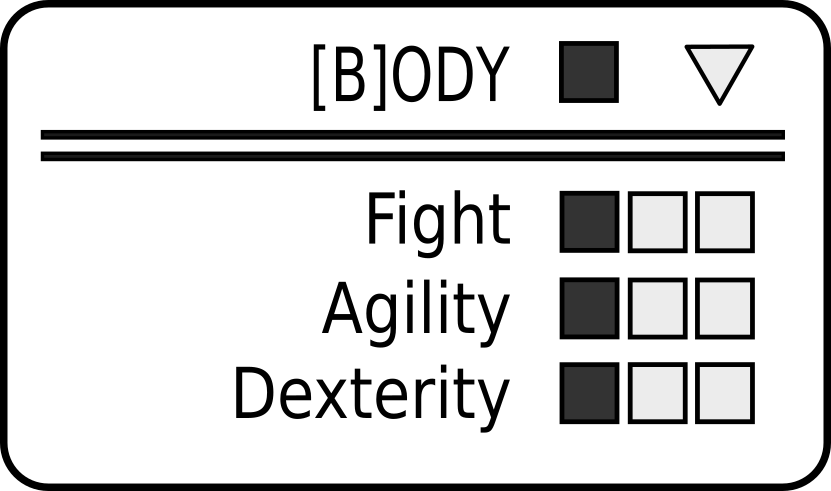
\includegraphics[width=0.80\textwidth]{images/character_body.png}
\end{column}

\begin{description}
    \item[\stat{Fight}] \stat{Fight} findet im Nah- und Fernkampf Anwendung. Es umfasst nicht nur den Angriff, sondern auch die 
        Verteidigung. Der Hintergrund bestimmt, in welcher Kampfart und mit welchen Waffen ein Charakter ausgebildet bzw.~ge"ubt ist.
    \item[\stat{Agility}] \stat{Agilit"at} umfasst Sportlichkeit, Fingerfertigkeit und die Nutzung aller Sinnesorgane. \stat{Agility} kann 
        im Kampf f"ur eine Flucht, das Wegtauchen in eine Deckung, aber auch zum Ausweichen von Schl"agen genutzt werden. F"ur das Ausweichen von Schl"agen kann alternativ auch \stat{Fight} genutzt werden.

        Die Fingerfertigkeit bei Reparaturen "uberschneidet sich mit den handwerklichen F"ahigkeiten, f"ur die auch \stat{Dexterity} genutzt werden kann.
    
        \stat{Agility} umfasst die Sinneswahrnehmungen Sehen, Tasten, Riechen und F"uhlen. Es kann z.B.~beim Durchsuchen von R"aumen angewendet werden. 
    \item[\stat{Dexterity}] \stat{Dexterity} umfasst handwerkliche F"ahigkeiten, die Bedienung von schwerem Ger"at sowie die Steuerung von 
        Fahrzeugen und Schiffen. Der spezifische Hintergrund des Charakters bestimmt die Auspr"agung und Anwendungsbereiche dieser F"ahigkeit.
\end{description}

\medskip
\begin{column}[l]{0.55}
    Das Attribut \stat{EMPATHY}, gruppiert alle sozialen F"ahigkeiten des Charakters. Es stehen folgende F"ahigkeiten zur Verf"ugung:
\end{column}
\begin{column}[r]{0.45}
    \centering
    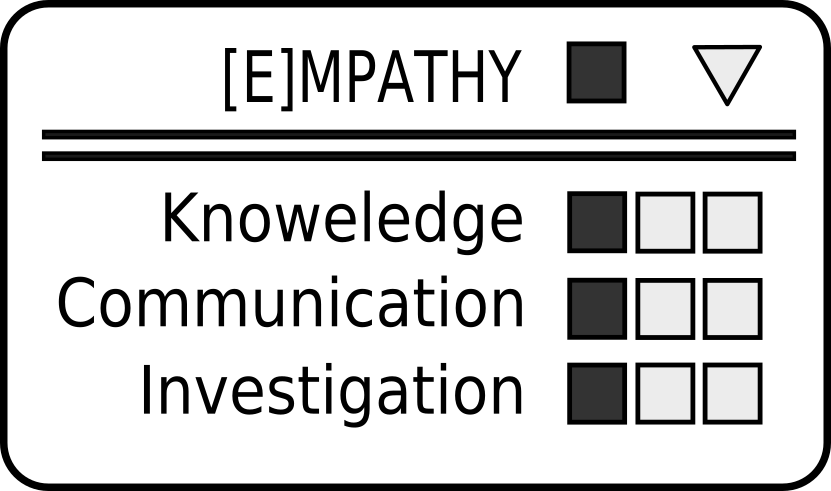
\includegraphics[width=0.80\textwidth]{images/character_empathy.png}
\end{column}

\begin{description}
    \item[\stat{Knowledge}] \stat{Knowledge} beschreibt das Allgemeinwissen und den "Uberblick "uber das aktuelle Geschehen.
        Dieses Wissen ist in der Regel auf den Kulturkreis und den Werdegang des Charakters beschr"ankt. Beispielsweise hat ein auf dem Mars aufgewachsener Charakter nur begrenztes Wissen "uber die russische Geschichte, es sei denn, er hat sich gezielt damit besch"aftigt.

        Ein Charakter mit einem hohen \stat{Knowledge}-Wert ist stets gut informiert und kennt die neuesten Entwicklungen, die f"ur sein Umfeld relevant sind.
    \item[\stat{Communication}] \stat{Communication} beschreibt die Kommunikationsf"ahigkeit des Charakters, also wie gut er mit anderen 
        Personen interagieren kann.

        Diese F"ahigkeit umfasst, wie gut der Charakter andere einsch"atzen, sich in sie hineinversetzen und sie gegebenenfalls manipulieren kann.

        \stat{Communication} umfasst die Kontaktnetzwerke des Charakters. Ein hoher \stat{Communication}-Wert erh"oht die Wahrscheinlichkeit, dass der Charakter jemanden kennt, der ihm bei einer Aufgabe helfen kann.
    \item[\stat{Investigation}] \stat{Investigation} bestimmt, wie effektiv ein Charakter Nachforschungen anstellen kann. Diese F"ahigkeit 
        erm"oglicht es ihm, Verborgenes zu entdecken.

        \stat{Investigation} findet sowohl in der realen als auch in der virtuellen Welt Anwendung.
\end{description}

\medskip
\begin{column}[l]{0.55}
    F"ur das Attribut \stat{EDUCATION}, das die Bildung und Fachkenntnisse des Charakters repr"asentiert, stehen folgende F"ahigkeiten zur Verf"ugung:

\end{column}
\begin{column}[r]{0.45}
    \centering
    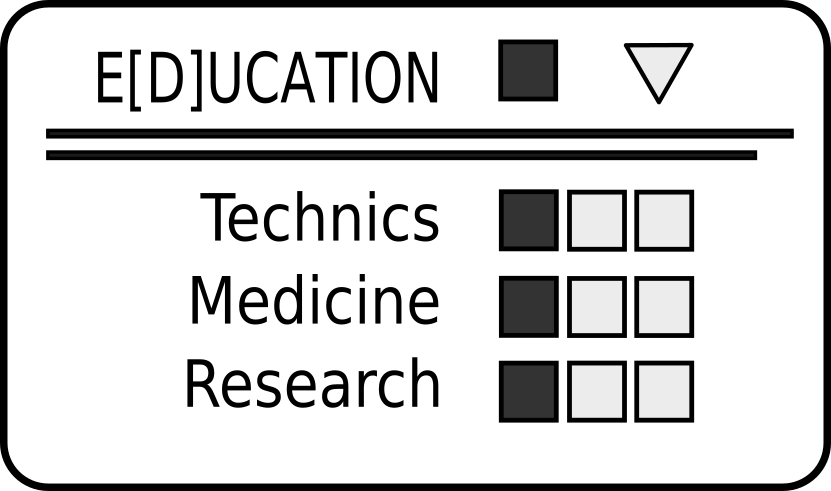
\includegraphics[width=0.80\textwidth]{images/character_education.png}
\end{column}

\begin{description}
    \item[\stat{Technics}] \stat{Technics} beschreibt das Wissen und Verst"andnis f"ur technische Systeme. Je nach \stat{BACKGROUND} kann das beispielsweise Raumfahrttechnik, Computertechnik oder "Ahnliches umfassen.
    \item[\stat{Medicine}] \stat{Medicine} beinhaltet medizinisches Wissen, einschlie\3lich Pharmakologie und Drogenkunde. 
    
        Diese F"ahigkeit umfasst T"atigkeiten als Arzt oder Sanit"ater sowie das Verst"andnis f"ur Abl"aufe in medizinischen Einrichtungen wie Krankenh"ausern. 
        
        Die Anwendung dieser F"ahigkeit ist abh"angig vom medizinischen \stat{BACKGROUND} des Charakters.
    \item[\stat{Research}] \stat{Research} umfasst Forschungskompetenz in Fachgebieten, basierend auf seinem \stat{BACKGROUND}, mit denen 
        der Charakter vertraut ist.
\end{description}

\underline{Anmerkung:} Wie die Beschreibungen zeigen, ist die Anwendbarkeit der F"ahigkeiten des Attributs \stat{EDUCATION} besonders abh"angig vom \stat{BACKGROUND} des Charakters. Die F"ahigkeit \stat{Research} kann beispielsweise nicht in allen wissenschaftlichen Bereichen angewendet werden, sondern nur in jenen, f"ur die der Charakter ausgebildet wurde.

\medskip
\begin{ruleexample}
    Die Gruppe fl"uchtet von einer Orbitalstation mit einem Wartungsshuttle, um sich auf einem Mond zu verstecken. Das Haupttriebwerk des Shuttles ist au\3er Betrieb. Um das Shuttle zu beschleunigen und auf die richtige Flugbahn zu bringen, wird ein Parabelflug geplant, der die Gravitation mehrerer Meteore in der Umgebung ausnutzt. Hierf"ur m"ussen alle Charaktere zusammenarbeiten:

\begin{description}
        \item[Celine ({Hintergrund Mathematikerin [D]})] Celine berechnet mithilfe ihrer mit drei W"urfeln ausgepr"agten F"ahigkeit 
            \stat{Research} eine Flugbahn.
        \item[Henk ({Hintergrund Navigator [E)})] Henk nutzt die von Celine berechnete Flugbahn, um mit seiner F"ahigkeit \stat{Knowledge} 
            die Flugparameter zu bestimmen.
        \item[Tom ({Hintergrund Shuttlepilot [B]})] Tom, der Pilot, bringt mit seiner F"ahigkeit \stat{Dexterity} das Shuttle mit den 
            Man"overd"usen aus dem Raumdock und folgt den von Henk bestimmten Flugparametern, um das Shuttle auf die richtige Flugbahn zu setzen.
    \end{description}
\end{ruleexample}

\newsubsection{Waffen}
\begin{column}[l]{0.55}
    Im Bereich \stat{WEAPONS} werden die Waffen eingetragen, die dem Charakter zur Verf"ugung stehen. Spielercharaktere verf"ugen "ublicherweise "uber eine halbautomatische Handfeuerwaffe. Abh"angig von der Profession des Charakters k"onnen zus"atzliche Waffen zur Verf"ugung stehen. Die Auswahl der Waffen ist mit dem Spielleiter abzustimmen.
\end{column}
\begin{column}[r]{0.45}
    \centering
    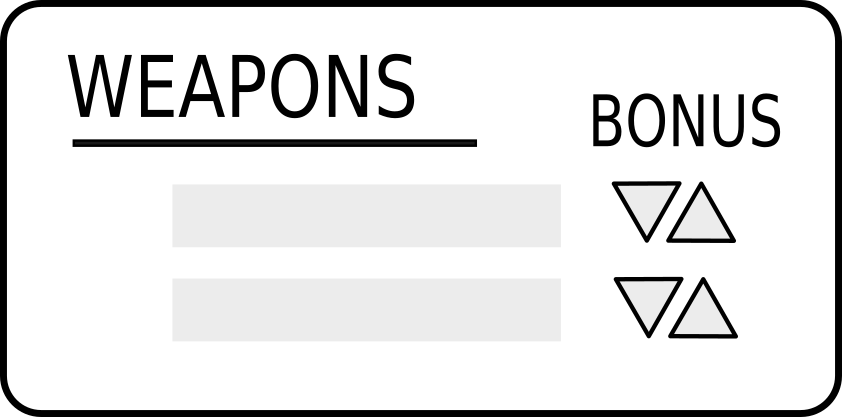
\includegraphics[width=0.80\textwidth]{images/character_weapons.png}
\end{column}
\medskip

Eine Auswahl an Waffen, beschrieben \cref{sec:weapons}, steht zur Verf"ugung. Dort sind auch die speziellen Eigenschaften der Waffen notiert. Wie Waffen im Rahmen des Regelwerks gruppiert werden findet sich \cref{sec:heavyweapons}.

Auf dem Charakterblatt sind neben jeder Waffe zwei Dreiecke angegeben. Bei Waffen, die schwer zu beherrschen sind, wird das nach unten zeigende Dreieck ausgef"ullt. Bei einer solchen Waffe werden Angriffe mit einem W"urfel weniger gew"urfelt (\emph{Malus}), jedoch mindestens mit einem W"urfel. Bei Waffen, die eine erh"ohte Trefferchance aufweisen, wird das nach oben zeigende Dreieck ausgef"ullt (\emph{Bonus}). Bei diesen Waffen wird mit einem zus"atzlichen W"urfel gew"urfelt.

\newsubsection{K"orperpanzerung}
\begin{column}[l]{0.55}
    Im Bereich \stat{ARMOR} werden die dem Charakter zur Verf"ugung stehenden K"orperpanzerungen und au\3ergew"ohnliche Kleidungsst"ucke wie individuelle Raumanz"uge eingetragen.
\end{column}
\begin{column}[r]{0.45}
    \centering
    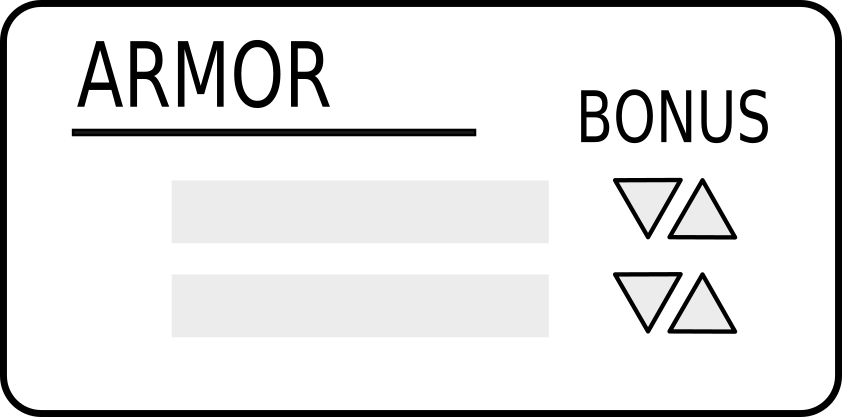
\includegraphics[width=0.80\textwidth]{images/character_armor.png}
\end{column}
\medskip

Eine Auswahl an K"orperpanzerungen ist \cref{sec:panzerung} gelistet. Dort sind auch die speziellen Eigenschaften der Panzerungen beschrieben.

Neben der Panzerung sind auf dem Charakterblatt zwei Dreiecke angegeben. Bei Kleidung, die den Charakter stark behindert und gleichzeitig unzureichenden Schutz bietet, wird das nach unten zeigende Dreieck ausgef"ullt. Bei solch einer Kleidung steht f"ur die Verteidigung ein W"urfel weniger zur Verf"ugung (\emph{Malus}). Bei Panzerungen, die den Charakter "uberdurchschnittlich gut sch"utzen, wie z.B. ein Servopanzer, wird das nach oben zeigende Dreieck ausgef"ullt. Bei einer solchen K"orperpanzerung steht ein W"urfel mehr zur Verf"ugung (\emph{Bonus}).

\newsubsection{Inventar}
\begin{column}[l]{0.55}
    Im Bereich \stat{INVENTORY} sind die pers"onlichen Habseligkeiten des Charakters aufgelistet. Zum Inventar z"ahlen auch K"orpermodifikationen wie Headware und modifizierte Gliedma\3en. Charaktere haben in der Regel ihre Ausr"ustung dabei. Die Gegenst"ande unter \stat{INVENTORY} sind diejenigen, die der Charakter "ublicherweise bei sich tr"agt. Diese werden in Absprache mit dem Spielleiter und unter Ber"ucksichtigung des Werdegangs des Charakters festgelegt.
\end{column}
\begin{column}[r]{0.45}
    \centering
    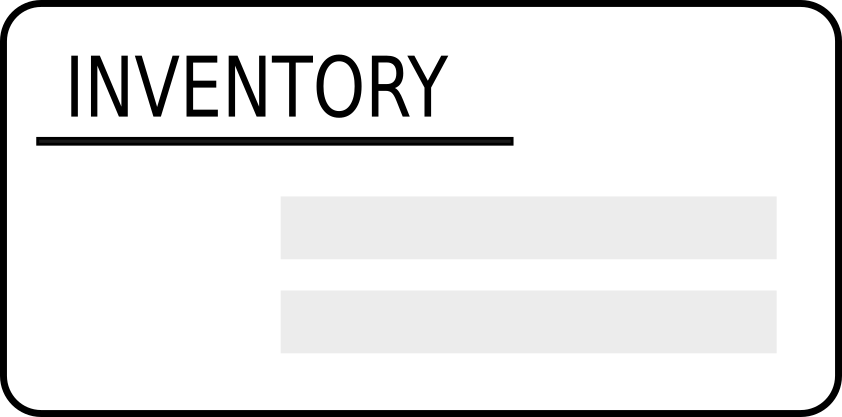
\includegraphics[width=0.80\textwidth]{images/character_inventory.png}
\end{column}

%% Copyright 2019 Bernd Haberstumpf
%% License: CC BY-NC
% !TeX spellcheck = de_DE
\newsection{Rassenbesonderheiten}

Den Spielern stehen Norms, Alpha-Mutanten und Omega-Krieger zur Auswahl. Bez"uglich dem Regelwerk gelten folgende Besonderheiten:

\begin{description}
    \item[Norms] Norms sind normale Menschen. Im Falle der Spielercharaktere handelt es sich normalerweise um Menschen mit einer 
        Hochschulausbildung im zivilen oder milit"arischen Sektor. Ihr St"arken liegen in den Attributen \stat{EMPATHY} und \stat{EDUCATION}. In einem dieser Bereiche k"onnen bis zu zwei zus"atzliche Punkte bei den F"ahigkeiten vergeben werden. 
        
        Die Charaktere k"onnen in ihrer Laufbahn eine leitende Stelle eingenommen haben und werden von Konzernmitarbeitern als Ansprechpartner wahrgenommen. 
        
        Die Charaktere haben in ihrer Vergangenheit m"oglicherweise hochwertige K"orpermodifikationen durchf"uhren lassen.
      
        Norms besitzen einen famili"areren Hintergrund, auch wenn der Kontakt abgebrochen sein mag, bestehen, wenn n"otig, Kontakte aus Schulzeit und Hochschulzeiten.
    \item[Alpha-Mutanten] Alpha-Mutanten sind in einer Zuchtfarm auf dem Mars als Arbeiter ausgebildet worden und haben keine Eltern. 
        Sie geh"oren der Arbeiterklasse an. Sie sind handwerklich gut ausgebildet. Aufgrund ihres genetischen Zuchtmaterials sind sie gr"o\3er, st"arker und widerstandsf"ahiger als Norms. Bei k"orperlichen T"atigkeiten wie auch bei K"orperbelastungen sollten diese k"orperlichen Besonderheiten bei den Auswirkungen von Aktionen ber"ucksichtigt werden. Die St"arken der Alpha-Mutanten liegen damit auf dem Attribut \stat{BODY}. Bei den entsprechenden F"ahigkeiten k"onnen dadurch jeweils bis zu zwei Punkte zus"atzlich ausgegeben werden. 
        
        Alphas werden als Teil der Zivilgesellschaft wahrgenommen und werden aufgrund ihrer meist umg"anglichen Art im extraterrestrischen Umfeld freundschaftlich behandelt und als zuverl"assig gesch"atzt. 
        
        Alpha-Mutanten sind im Normalfall mit dem Leben in Schwerelosigkeit vertraut. Alpha-Mutanten haben eine handwerkliche und meist eine logistische Ausbildung erhalten. 
        
        Sie haben innerhalb ihrer Zuchtreihe jeweils eine eigene Sprache entwickelt und k"onnen sich damit mit ihren ``Artgenossen'' aber auch anderen Alpha-Mutanten, unverst"andlich f"ur Norms und Omega-Mutanten unterhalten. 
    \item[Omega-Krieger] Omega-Krieger sind entweder auf dem Mars oder in Zuchtfarmen im erdnahen Orbit aufgewachsen. Sie sind   
        gr"o\3er und widerstandsf"ahiger als Alpha-Mutanten und Norms. Bei allen k"orperlichen Aktionen und Folgen von Verletzungen m"ussen diese "uberlegenen Eigenschaften ber"ucksichtigt werden. Ihre St"arke im W"urfelsystem liegt wie bei Alpha-Mutanten im Attribut \stat{BODY}. Hier k"onnen auf alle F"ahigkeiten bis zu zwei Punkte vergeben werden. 
        
        Omega-Krieger werden von klein auf den Krieg vorbereitet und ausgebildet. Nah- und Fernkampff"ahigkeiten sind vorauszusetzen. 
        Omega-Krieger sind mit milit"arischen K"orpermodifikationen ausgestattet. Omega-Krieger haben eine strategische und logistische Ausbildung f"ur Krisensituationen erhalten. Sie sind f"ur die m"uhelose Bewegung in Schwerelosigkeit vorbereitet. Sie haben auch eine medizinische Ausbildung als Sanit"ater erhalten. Viele Omega-Krieger sind ausgebildete Piloten oder haben eine Ausbildung als Schiffskommandant absolviert. 
        
        Aufgrund ihrer genetischen Programmierung sind Omega Mutanten leicht reizbar und gehen schnell offensiv mit einer Provokation oder einer Bedrohung um. Sie unterliegen deshalb dem \stat{FLAW} ``reizbar''. Von anderen Personen werden sie oft als militanten Bedrohung wahrgenommen.

        Omega-Krieger sind in den meisten F"allen Teil einer Armee, d.h. sie arbeiten als Soldaten oder S"oldner, in den meisten F"allen f"ur einen Konzern. In den Wirren des letzten Jahrhunderts sind aber auch eine Reihe von Omega-Kriegern desertiert oder ihre Einheiten wurden aufgel"ost.
\end{description}

\underline{Anmerkung:} Eine komplette "Ubersicht "uber alle Rassen findet sich \cref{sec:humanraces}.

%% Copyright 2019 Bernd Haberstumpf
%% License: CC BY-NC
% !TeX spellcheck = de_DE
\newsection{Kampf und Verletzungen}

Im Alltag eines Helden l"asst sich eine Auseinandersetzung nicht immer friedlich l"osen, und es kommt zum Kampf. In diesem Kapitel werden K"ampfe zwischen Personen und die Auswirkungen von Verletzungen beschrieben.

Eine Aktion in einem Kampf umfasst eine ganze \emph{Kampfszene}. Eine solche Kampfszene kann z.B. ein Nahkampfgefecht, ein Schusswechsel oder auch ein Ausweichman"over sein. Der Spieler beschreibt, wie er k"ampfen m"ochte und welches Ziel er in der Kampfszene erreichen m"ochte: M"ochte er einen oder mehrere Gegner mit Tritten zu Fall bringen, in Deckung hechten oder einen fl"uchtenden Gegner niederschie\3en?

Daraufhin wird gew"urfelt. K"ampfe sind normalerweise \textbf{vergleichende W"urfe} mit der Schwierigkeit \textbf{Einfacher Wurf}. Entschlie\3t sich ein Charakter, seinen Gegner \textbf{anzugreifen}, w"urfelt er mit seiner F"ahigkeit \textbf{Fight}. Beschr"ankt sich der Charakter auf \textbf{Verteidigung}, wird je nach Situation entweder mit \textbf{Fight} oder \textbf{Agility} gew"urfelt. Auf \textbf{Agility} wird gew"urfelt, wenn der Charakter einem Angriff ausweichen will.

\begin{ruleexample}
    Hektor und der Minenarbeiter Fury, ein kr"aftiger Alpha-Mutant, sind aneinander geraten. Fury schl"agt zu. Hektor sieht sich unterlegen und versucht zu fliehen.

    Fury w"urfelt auf \stat{Fight}. Hektors eingesetzte F"ahigkeit ist \stat{Agility}. Beide haben zwei W"urfel zur Verf"ugung. Im Rahmen eines vergleichenden Wurfs w"urfelt Fury mit einem W"urfel und erzielt eine \ssdice{4}, Teilerfolg. Furys Schl"age sind kr"aftig und gut gezielt, aber Hektor schafft es immer wieder, gekonnt abzutauchen, und steckt nur leichte Treffer ein.

    Hektor versucht, sich aus dem Kampf zu l"osen und die Flucht anzutreten. Er w"urfelt mit \stat{Agility}, reduziert durch Furys Angriffswert \stat{Fight}. Er w"urfelt ebenfalls mit einem W"urfel und erzielt eine \ssdice{5}, Teilerfolg. Hektor bringt sich auf Abstand und entscheidet sich, Fury zu beruhigen.
\end{ruleexample}

\newsubsection{Kampf mit mehreren Personen}
Oft sind an K"ampfen mehrere Personen beteiligt. Wie bei anderen Aktionen k"onnen Angreifer oder Verteidiger ihre Kr"afte b"undeln, um ihre Erfolgschancen zu erh"ohen. Das B"undeln wird \cref{sec:bundleforce}. Sowohl die Angreifer als auch die Verteidiger k"onnen ihre W"urfel b"undeln.

\newsubsection{Nahkampf}
Im Nahkampf treten Personen waffenlos oder mit Hieb- oder Stichwaffen gegeneinander an.

Im Folgenden sind einige spezielle Nahkampfsituationen beschrieben:

\begin{description}
    \item[Fixieren] Ein Angriff, um einen Gegner festzuhalten und bewegungsunf"ahig zu machen. Der Gegner ist dann kampfunf"ahig, kann sich 
        jedoch m"oglicherweise in einer sp"ateren Kampfszene befreien. Um einen Gegner zu fixieren, wird ein \textbf{voller Erfolg} ben"otigt. Ein Teilerfolg k"onnte bedeuten, dass der Gegner zwar nicht fl"uchten kann, aber noch nicht vollst"andig kampfunf"ahig ist.
    \item[Entwaffnen] Dem Gegner eine Waffe zu entrei\3en oder sie ihm zu entwinden, erfordert einen \textbf{vollen Erfolg}. Ein Teilerfolg 
        kann den Schaden des Angriffs verringern.
    \item[Schl"agerei] An einer Schl"agerei k"onnen viele Personen beteiligt sein. Aufgrund der Enge, k"onnen jedoch immer maximal drei 
        Personen ihre Angriffe b"undeln.
\end{description}

\newsubsection{Fernkampf}
Fernkampf bezieht sich auf Angriffe mit Wurfwaffen, Schusswaffen, Granaten und Plasmaschleudern. Der Angreifer w"urfelt mit der F"ahigkeit \stat{Fight}, um anzugreifen.

Folgende Besonderheiten m"ussen ber"ucksichtigt werden:

\begin{description}
    \item[Ausweichen] Um einem Fernkampfangriff auszuweichen, muss der Verteidiger in der Regel bereits in Bewegung sein, Haken schlagen 
        oder in Deckung hechten. Um auf einen Fernkampfangriff zu reagieren, wird mit der F"ahigkeit \textbf{Agility} gew"urfelt.
    \item[Duell] Ein Angreifer, der eine Fernkampfwaffe nutzt, kann normalerweise anderen Angriffen kaum ausweichen. Um dennoch auf 
        einen Gegenangriff zu reagieren, ist ein \textbf{Risikowurf} erforderlich.
    \item[Point-Blank] Ein Angreifer, der einen Gegner ohne Deckung aus kurzer Distanz bedroht, hat leichtes Spiel. Er w"urfelt seinen 
        Angriff mit einem \textbf{Alltagswurf}. Der Angegriffene kann entweder einen Nahkampf-Gegenangriff versuchen oder sich mit einer schnellen Bewegung aus der Schusslinie bringen, wenn ihm der Sch"utze Auge-in-Auge gegen"ubersteht. In diesem Fall w"urfelt er einen \textbf{Risikowurf} als Gegenreaktion.
    \item[Deckung] Ein Verteidiger, der in teilweiser Deckung steht, ist schwerer zu treffen. Die Verteidigung erh"alt einen \textbf{Bonus}  
        von einem W"urfel, sofern die R"ustung diesen Bonus nicht bereits bietet.
\end{description}

\newsubsection{Schaden}\anchor{sec:schaden}
Bei K"ampfen und auch in anderen Situationen kann ein Charakter verletzt werden. Verletzungen werden nicht wie in anderen Rollenspielen durch Lebenspunkte festgehalten. Stattdessen bestimmt der Spielleiter basierend auf dem Angriff, der Verteidigung, der Panzerung sowie den Umst"anden, die zur Verletzung f"uhren, welche Art von Verletzung der Charakter erleidet. Die Auswirkung einer Verletzung legt der Spielleiter fest.

\begin{column}[l]{0.58}
    Wird der Charakter im Kampf oder bei einer sonstigen T"atigkeit verletzt, wird unter \stat{DAMAGE} die zugezogene Verletzung notiert. Es wird zwischen \textbf{leichtem} und \textbf{schwerem Schaden} unterschieden. Bei schweren Verletzungen ist ein Konstitutionswurf notwendig, damit der Charakter handlungsf"ahig bleibt. Werden schwere Sch"aden nicht behandelt oder setzt sich der Charakter weiterhin k"orperlicher Belastung aus, kann er ebenfalls handlungsunf"ahig werden. In diesem Fall k"onnen weitere Konstitutionsw"urfe erforderlich werden. Ein Konstitutionswurf ist in der Regel ein \textbf{einfacher Wurf} auf \stat{CONST}.
\end{column}
\begin{column}[r]{0.42}
    \centering
    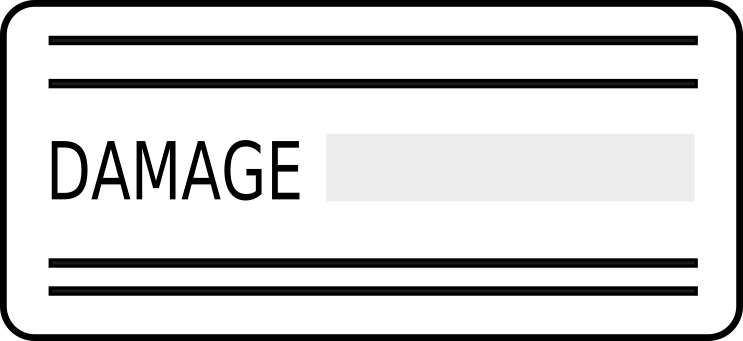
\includegraphics[width=0.80\textwidth]{images/character_damage.png}

    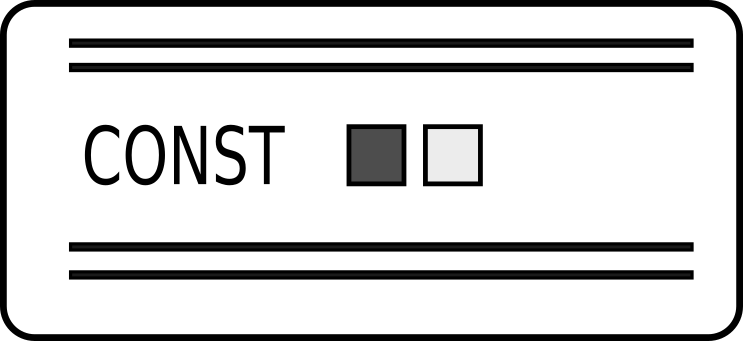
\includegraphics[width=0.80\textwidth]{images/character_const.png}
\end{column}
\smallskip

Schwere Verletzungen in Verbindung mit einem erfolglosen Konstitutionswurf k"onnen zum Tod f"uhren. Die Verletzung muss sofort behandelt werden, andernfalls f"uhrt sie unweigerlich zum Exitus. Ein sterbender Charakter kann jedoch wiederbelebt werden. Die Medizin im 23. Jahrhundert ist, wie \cref{sec:helden} beschrieben, weit fortgeschritten. K"orpermodifikationen k"onnen dabei helfen, den Charakter am Leben zu halten. Ein Erste-Hilfe-Kit enth"alt Ausr"ustung zur Wiederbelebung und Stabilisierung.

\newsubsection{Kleine, Leichte, schwere und Bet"aubungswaffen}\anchor{sec:heavyweapons}

Im Rahmen des Regelwerks wird zwischen kleinen, leichten und schweren Waffen unterschieden.

\begin{description}
    \item [Kleine Waffen] Unter kleinen Waffen werden alle Nahkampfwaffen und Handfeuerwaffen verstanden. Alle Panzerungen im n"achsten 
        Kapitel \cref{sec:panzerung} bieten effektiven Schutz gegen kleine Waffen.
    \item[Leichte Waffen] Unter leichte Waffen fallen vollautomatische Gewehre wie Railguns und Handgranaten. Gegen leichte Waffen bieten 
        Panzerungen, au\3er einem Servopanzer, nur begrenzten Schutz.
    \item[Schwere Waffen] Unter schwere Waffen fallen Plasmaschleudern, Granatwerfer, Raketenwerfer und alle Fahrzeug-gest"utzten 
        Waffensysteme. Auch ein Teiltreffer ist in den meisten F"allen fatal. Nur ein Servopanzer bietet Schutz gegen einen indirekten Treffer (Teilerfolg).
    \item[Bet"aubungswaffen] Unter Bet"aubungswaffen versteht man Waffen, die einen Gegner au\3er Gefecht setzen, ohne ihn schwer zu 
        verwunden.
        
        Eine effektive Munition dieser Kategorie sind Schockprojektile. Hierbei handelt es sich um nicht penetrierende Projektile, die beim Aufprall auf das Ziel kurzzeitig einen starken Stromsto\3 abgeben, der zu Muskelkr"ampfen, Bewusstlosigkeit und zum Ausfall von elektronischen Ger"aten wie Cyberware f"uhren kann. Gegen Schockprojektile bietet nur ein Servopanzer effektiven Schutz. Andere Panzerungen bieten nur begrenzten Schutz.
\end{description}

\underline{Anmerkung:} Die hier verwendeten Begriffe entsprechen nicht den offiziellen Bezeichnungen der UN.

\newsubsection{Panzerung}\anchor{sec:panzerung}
Um sich gegen Angriffe zu sch"utzen, kommt Panzerung ins Spiel. Eine Panzerung sch"utzt recht zuverl"assig vor kleinen Waffen. Kritisch sind ungesch"utzte K"orperteile. Ein Treffer auf ungesch"utzte K"orperteile erfordert einen \textbf{vollen Erfolg}.

Folgende Panzerungen kommen im C23-Universum zum Einsatz:

\begin{description}
    \item[Schusssichere Weste und Helm] Eine schusssichere Weste und ein Helm bieten bereits einen effektiven Schutz gegen Feuerwaffen. Sie 
        sch"utzen den Torso und Teile des Kopfes effektiv vor Stichwaffen und Projektilen und bieten auch Schutz gegen stumpfen Waffen. Ein Treffer auf Weste und Helm hinterl"asst Prellungen, verursacht jedoch keine gr"o\3eren Verletzungen.
    \item[Kampfanzug] Noch besseren Schutz bietet ein Kampfanzug. Ein Kampfanzug sch"utzt alle Teile des K"orpers, aber er bietet keinen 
        vollst"andigen Schutz vor Schusswaffen oder Schl"agen. Bewegliche Teile wie Gliedma\3en sind weniger gut gesch"utzt. Nur ein \textbf{herausragender Erfolg} trifft ein schlecht gesch"utztes K"orperteil.
    \item[Servopanzer] Ein Servopanzer ist ein hydraulisch unterst"utztes Ganzk"orper-Exoskelett mit eingebautem Raumanzug und 
        Waffensystemen. Treffer mit einer Nahkampfwaffe oder einer Bolzenpistole sind bei einem Servopanzer wirkungslos. Selbst die schw"acher gesch"utzten K"orperteile bieten eine Schutzwirkung, die mit einer schusssicheren Weste vergleichbar ist.
\end{description}


%% Copyright 2019 Bernd Haberstumpf
%% License: CC BY-NC
% !TeX spellcheck = de_DE
\newsection{Cyberkampf}\anchor{sec:cyberkampf}
Cyberkampf ist der Kampf im ComNetz. Ein Charakter kann sich in das ComNetz mittels eines station"aren Terminals, eines Computers oder seines ComLinks einloggen. Weitaus effektiver ist jedoch das vollsensorische Eintauchen mittels eines Kontrollmoduls. Der Charakter taucht dann mit all seinen Sinnen in die virtuelle Realit"at des Datennetzes ein. Mittels Gedankenkontrolle lassen sich Befehle absetzen, und Informationen k"onnen "uber alle Sinnesorgane aufgenommen werden. F"ur diese Art des Einstiegs ins Netz ist eine breitbandige Kabelverbindung notwendig.

Zur Informationsbeschaffung oder "Uberwachung im Netz k"onnen Agentensysteme mit Auftr"agen losgeschickt werden. Andere Systeme im Netz k"onnen "uber eine Cyberattacke, unterst"utzt durch Agentensysteme und Viren, angegriffen werden.

Auch das ComLink zusammen mit dem Personal Area Network (PAN) eines Netzteilnehmers oder das Kontrollmodul sind Systeme im Netz, die angegriffen werden k"onnen. Eingespeiste Viren k"onnen die Headware des Teilnehmers beeintr"achtigen und dadurch Sinneswahrnehmungen beeinflussen, Hormoneinspeisungen einleiten oder k"unstliche K"orperfunktionen st"oren. Firewallsoftware sch"utzt alle Formen von Systemen im Netz vor Cyberattacken.

Eine Cyberattacke wird wie eine physische Attacke durch vergleichende W"urfelw"urfe durchgef"uhrt. Cyberangriffe und das Programmieren von Viren und Agentensystemen werden mit der F"ahigkeit \textbf{Technics} gew"urfelt.

%% Copyright 2019 Bernd Haberstumpf
%% License: CC BY-NC
% !TeX spellcheck = de_DE
\newsection{Psychonauten}
Psychonauten, wie \cref{sec:technology} beschrieben, k"onnen mithilfe spezieller Ausr"ustung in das Gehirn einer anderen Person eindringen. "Ahnlich wie beim Eintauchen in das ComNetz besteht dann eine vollsensorische Verbindung zwischen beiden Personen. Der Psychonaut ``denkt'' quasi im Gehirn des anderen mit. Zun"achst dringt der Psychonaut in die oberfl"achlichen Gedanken des Hier und Jetzt ein, kann aber auch tiefer in das Unterbewusstsein vordringen, um Wissen und Gef"uhle zu erkunden. Der Psychonaut kann spezifische Informationen anfordern und nimmt diese "ahnlich wie in einem Traum durch Bilder und Sinneseindr"ucke wahr.

Ein Gehirnscan wird mit der F"ahigkeit \textbf{Research} gew"urfelt. Das Opfer des Gehirnscans kann sich mit \textbf{Empathy} bei dem vergleichenden Wurf verteidigen, im Falle eines Psychonauten ebenfalls mit \textbf{Research}.

Ein Gehirnscan ist sowohl f"ur das gescannte Opfer als auch f"ur den Psychonauten gef"ahrlich. Wehrt sich das Opfer bei einem Tiefenscan und erzielt einen Misserfolg, kann sein Gehirn psychischen Schaden erleiden. Auf der anderen Seite ist die Gehirnverbindung bidirektional. Ein Misserfolg beim Scan kann dazu f"uhren, dass das Opfer selbst Informationen aus dem Gehirn des Psychonauten erh"alt oder dass der Psychonaut psychischen Schaden nimmt.

Die F"ahigkeit ``Psychonaut'' ist ist ein \stat{Merit}, das in Absprache mit dem Spielleiter vergeben werden kann. Psychonauten sind in ihrer F"ahigkeit ausgebildet. Psychonaut wird ebenfalls unter \stat{BACKGROUND} als ``Psychonaut[D]'' vergeben.

%% Copyright 2019 Bernd Haberstumpf
%% License: CC BY-NC
% !TeX spellcheck = de_DE
\newsection{Raumkampf}
Bei einer Auseinandersetzung im Weltall k"onnen K"ampfe mit den \cref{sec:spaceship} beschriebenen Schiffsklassen ausgefochten werden.

Den Charakteren stehen "ublicherweise F"ahren, Frachter oder eventuell auch eine Korvette zur Verf"ugung. Korvetten und J"ager sind mit Railguns oder Gau\3kanonen ausgestattet, gelegentlich auch mit Raketen oder Torpedos. Mehrere Hundert Meter gro\3e Kriegsschiffe wie Fregatten, Schlachtkreuzer und Flottentr"ager sind mit Railguns, Gau\3kanonen, Raketen und Torpedos best"uckt. Railguns werden bei Schiffen gr"o\3er als eine Korvette aufgrund ihrer hohen Feuerfrequenz prim"ar als Verteidigungswaffen genutzt. Sonden k"onnen zur Aufkl"arung "uber gro\3e Entfernungen eingesetzt werden.

Technisch besteht ein Schiff "uberwiegend aus einem Fusionstriebwerk als Hauptantrieb, einer Reihe von Steuerungstriebwerken, einem Lebenserhaltungssystem und einer gro\3en Anzahl von Sensoren. Alle Systeme, bis auf Triebwerke, sind mit Redundanzsystemen ausgestattet. Da die Mannschaft im freien Raum komplett auf sich allein gestellt ist, k"onnen die meisten technischen Systeme eines Schiffs autonom repariert und ausgetauscht werden. Ein Weltraumspaziergang ist f"ur die Crew eines Schiffes kein au\3ergew"ohnlicher Vorfall und kann auch bei hoher Fluggeschwindigkeit durchgef"uhrt werden. Ein Gro\3teil der Zeit befindet sich ein Schiff im Driftflug, d.h. mit ausgeschalteten Triebwerken. Es herrscht Schwerelosigkeit an Bord. Nur unbedingt notwendige Systeme sind aktiv. Der Reaktor des Haupttriebwerks kann innerhalb einer Minute hochgefahren werden und bietet dann ein Vielfaches an Schub im Vergleich zu einem klassischen Raketenantrieb. Ein Fusionstriebwerk wie auch die Steuerd"usen ben"otigen Treibmasse, allerdings in deutlich geringerer Menge als bei heutigen Raketen.

Im freien Raum sind die Gegebenheiten viele Stunden vor einem Zusammentreffen einsehbar. Der taktische Computer des Schiffes zeigt alle "uber die Sensorik erfassten Daten in einer 3D-Ansicht an. Auf dem Display oder eingeblendet im Gehirn sind die aktuellen und prognostizierten Flugbahnen von Schiffen, Planeten, Monden und anderen Himmelsk"orpern einsehbar, sofern sie erfasst werden k"onnen.

Ein strategisches Planen von Raumk"ampfen auf einem Schlachtplan w"are m"oglich. Ist der Kampf jedoch nicht der Fokus der Geschichte, sollten nur einige kurze Kampfszenen ausgespielt werden. Die Schiffskontrolle und die Kontrolle der Waffensysteme werden durch die F"ahigkeit \textbf{Dexterity} abgebildet. F"ur notwendiges Fachwissen bei Reparaturen wird die F"ahigkeit \textbf{Technics} herangezogen. F"ur Flugplanung und Raumkartografie wird die F"ahigkeit \textbf{Knowledge} ben"otigt. F"ur einen Au\3enspaziergang w"urfelt man auf \textbf{Dexterity}.



